\documentclass[a4paper]{article}

\usepackage[pdftex]{graphicx}
\usepackage{a4wide}
\usepackage{hyperref}
\usepackage{times}
\usepackage{mdwlist}
\usepackage{molto_titlepage}

% TODO: get UTF to work in biblio (Normunds' citation)
\usepackage[utf8]{inputenc}
\usepackage[T1]{fontenc}

\graphicspath{{./images/}}

\def\xp#1{\texttt{#1}}
\newcommand\ace{Attempto Controlled English}

\begin{document}

\begin{moltotitlepage}
\id{D11.1}
\title{ACE Grammar Library}
\author{John J. Camilleri, Norbert E. Fuchs, Kaarel Kaljurand}
\distributionLevel{Public}
\type{Prototype}
\version{1.1 (2012-06-27)}
\dateContractual{M27}
\dateActual{2012-06-01}
\siteResponsible{UZH}
\siteContributors{UGOT}
\end{moltotitlepage}

\hyphenation{alpha-numeric}
\hyphenation{ex-pe-ri-ment-al}
\hyphenation{in-de-pend-ent}

\begin{abstract}
This report describes the implementation of a large part of the
Attempto Controlled English (ACE) syntax ---
the subset of ACE that is accepted by the AceWiki semantic wiki system ---
in Grammatical Framework (GF) and making it available via 10
languages that are supported by the GF Resource Grammar Library (RGL).
As a result, ACE becomes available in multiple languages, making
ACE-based knowledge representation possible also in languages other than
English.
Additionally, the GF-based implementation of the ACE language provides
ACE users with new (GF-based) editing tools.
\end{abstract}

\clearpage
\thispagestyle{empty}
\tableofcontents

\clearpage
\setcounter{page}{1}
\section{Introduction}

\ace{} (ACE) \cite{fuchs:reasoningweb2008} is a controlled natural language
(CNL), concretely a general purpose
first-order language (FOL)
with English syntax.
ACE can be viewed as both a natural language understandable by every
English speaker, and a formal language with a precisely defined
syntax and semantics understandable by automatic theorem provers.
ACE texts are deterministically interpreted
via Discourse Representation Structures (DRS) \cite{kamp:drt1993}.
The syntactically legal sentence structures and their
unambiguous interpretation are explained as
\emph{construction} and \emph{interpretation} rules
in the end-user documentation.
The ACE toolchain includes a parser that maps ACE sentences into a concrete
DRS form \cite{ifi-2010.0010} and further into formats supported by existing
automatic reasoners (e.g. OWL, SWRL, TPTP).

The current version 6.6 of ACE offers many language constructs, the most
important of which are
countable and mass nouns (`man', `water');
proper names (`John');
generalised quantifiers (`at least 2');
indefinite pronouns (`somebody');
intransitive, transitive and ditransitive verbs (`sleep', `like', `give');
negation, conjunction and disjunction of
noun phrases, verb phrases, relative clauses and sentences;
and anaphoric references to noun phrases through
definite noun phrases, pronouns, and variables.
End-users working with ACE can specify a lexicon that maps English
wordforms of nouns, verbs, adjectives, adverbs and prepositions
into logical atoms,
which the users
can interpret as they wish, but otherwise the ACE grammar or its mapping to
DRS cannot be changed.

The full ACE specification describes a language which goes beyond the
expressivity of many popular knowledge representation languages. Therefore,
several subsets of ACE have been defined to allow for a more direct
mapping to and from these languages. The most explicitly defined subset
is the language used in the AceWiki semantic wiki system
\cite{kuhn2010doctoralthesis}, which closely corresponds to the OWL ontology
language \cite{OWL_2_Web_Ontology_Language_Document_Overview}.

Grammatical Framework (GF) \cite{ranta:book2011}
is a framework for defining multilingual grammars.
GF provides a functional programming language in which
the grammar author implements an abstract grammar and its corresponding
concrete grammars and by doing that
describes a bidirectional mapping between concrete language strings and
their corresponding abstract syntax trees. This architecture supports
multilingual translation as strings of one concrete language can be parsed into
abstract trees which can be further linearised as strings in another concrete
language.

GF is an expressive formalism optimised to handle natural language features
like morphological variation, agreement, long-distance dependencies, etc.
GF comes with various tools that
cover grammar authoring, compatibility with many popular programming languages,
conversion into other grammar formats, and a reusable grammar library covering
many world natural languages and providing a language-neutral application
programming interface (API) to a large
number of linguistic categories (e.g. NP, VP) and constructs
(e.g. the combination of NP and VP into a sentence).

The purpose of this report is to study whether it is possible and useful to
implement the grammar of ACE in GF, with the main goal of turning ACE into
a multilingual CNL.
In section \ref{section:Goals_and_requirements} we describe the goals and
requirements that a GF-based implementation of ACE should meet;
in section \ref{section:Existing_work} we point out two existing
GF implementations of ACE;
in section \ref{section:ACE_in_GF} we describe our implementation;
in section \ref{section:Multilinguality} we describe the most important feature
of this implementation, namely multilinguality;
in section \ref{section:Evaluation} we evaluate the implementation by comparing
it to existing implementations of the ACE grammar and discuss the multilingual
representations of ACE sentences;
in section \ref{section:Conclusions} we summarise the work and
describe its possible extensions.

The developed grammar as well as the test sets, development tools and
documentation are available under the LGPL license on the GitHub repository

\begin{quote}
\url{https://github.com/Attempto/ACE-in-GF}
\end{quote}

\section{Goals and requirements}
\label{section:Goals_and_requirements}

The overall goal of this work is to make ACE available to users who have little
English skills by turning ACE-based systems like
AceWiki \cite{kuhn2010doctoralthesis} multilingual. This allows users
to create and consume content whose native format is a formal language
(specifically a FOL-based language) in multiple natural languages
via an ACE-based interlingua (see figure \ref{fig:languages}).
Also, having a GF implementation of the ACE language would
provide ACE users with (editing) tools that are based on the GF technology,
offering e.g. look-ahead editing, embeddable grammars, conversion into
speech recognition grammar formats, etc.

\begin{figure}[ht]
\centering
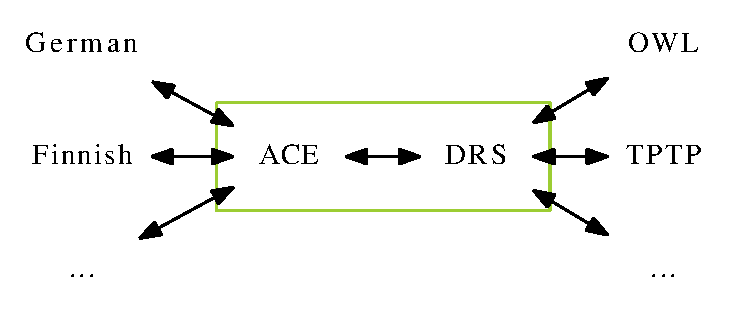
\includegraphics[width=0.7\textwidth]{languages}
\caption[Languages]
{Bidirectional mapping between a formal language like OWL and a natural
language like Finnish facilitated by the multilingual GF-implementation of
ACE and various mappings between ACE and other formal languages.}
\label{fig:languages}
\end{figure}

%Our main research questions are:
%
%\begin{itemize}
%\item what are the features and benefits of a general purpose multilingual
%controlled natural language?
%\item is it technically possible to implement the ACE syntax in GF,
%and what are the benefits of such an implementation?
%\end{itemize}

Our goal is to demonstrate that a large fragment of the ACE syntax
can be implemented in a language-neutral way and ported to a large number
of different natural languages.
% (including ACE itself).
This involves showing that

\begin{itemize}
\item the ACE-language implementation in the resulting grammar matches
precisely the chosen ACE subset (in our case the AceWiki subset)
and can be parsed unambiguously, facilitating a further unambiguous mapping
to other natural or formal languages;
\item the resulting grammar remains maintainable, i.e. extending and modifying
it to reflect possible changes in the ACE specification is straight-forward;
\item multilingual translations of the same abstract tree preserve the precise
and unambiguous meaning assigned to the ACE sentences by the ACE interpretation
rules, i.e. users reading the translations understand them in the same way
as users reading the original ACE sentences;
\item adding support for new languages is straight-forward and requires little
extra work.
\end{itemize}

Note that this report describes the implementation of the ACE syntax,
i.e. not its DRS mapping. The latter is not necessary for the purposes of a
multilingual grammar. As most usages of ACE involve its DRS mapping, also
most usages of the our GF implementation
will have to combine it with the existing ACE parser, which provides the
mapping to DRS and further into other logical forms (including a verbalisation
back into ACE which can be used to paraphrase the original text).


\section{Existing work}
\label{section:Existing_work}

Our work builds on \cite{ranta:cnl2009_revised} which implements the syntax
of ACE v6.0 (by following \cite{ACE_6.0_Construction_Rules}) and makes it
available in 7 languages (English, French, German, Italian, Swedish, Finnish
and Urdu) via the GF Resource Grammar Library (RGL) \cite{ranta:lilt2009}.
Our goal is to update this implementation to ACE v6.6, make it precisely
cover a large subset of ACE, and increase the number of natural languages to
which the grammar is ported.

Another existing work that implements ACE in GF is
``ACE compliant controlled Latvian for ontology authoring and verbalisation''
\footnote{\url{http://valoda.ailab.lv/cnl/}}
\cite{gruzitis:phd}. The goal of this work is to bidirectionally map Latvian
language sentences to OWL axioms and queries. The developed system
does not expose ACE to the end-user and only treats it as a
machine-readable intermediate format that provides access to the ACE tools
(specifically the bidirectional OWL converter).
It therefore does not have to deal with the
generation of correct ACE wordforms.
The system is also not built with multilinguality in mind
(i.e. it does not use the general GF RGL APIs). The developed ACE grammar
cannot thus serve easily as a starting point of the work described in this
report.


\section{Implementation of ACE in GF}
\label{section:ACE_in_GF}

Rather than directly building a grammar for the
full ACE v6.6 \cite{ACE_6.6_Construction_Rules}, we chose to focus
on the subset of ACE that is used by the AceWiki semantic wiki system. The
resulting grammar can be seen as a core module which can be used by AceWiki
without any change and which can be extended by a separate grammar
towards full ACE as need arises. The AceWiki subset is a relatively expressive
fragment of ACE, roughly matching the expressivity of the OWL ontology
language
\cite{OWL_2_Web_Ontology_Language_Document_Overview}
without data properties.
This makes the subset relevant in (Semantic Web) ontology editing applications.
The other benefit of the AceWiki subset is that it is formally defined by a
Codeco grammar \cite{kuhn:cnl2010_revised}
\footnote{\url{http://attempto.ifi.uzh.ch/site/docs/acewikijava/ch/uzh/ifi/attempto/acewiki/aceowl/acewiki_grammar.html}},
which provides both parsing and generation and thus gives us an excellent
reference implementation against which we can easily test our GF-based
implementation.
With Codeco we can perform exhaustive generation of syntactically legal
sentences. Also the Codeco grammar can be used to implement look-ahead
editors, similarly to GF, which provides for us another point of comparison.

\subsection{Comparison of Codeco and GF}
\label{subsection:Codeco}

Codeco is a unification grammar formalism with special support for describing
anaphoric references. For example, the following (simplified) rules

\small
\begin{quote}
\begin{verbatim}
simple_sentence => 'there is' np[pl:-, def:-, exist:+]
np[def:+] => 'the' noun[noun:Noun] <[type:noun, noun:Noun] >[type:ref]
\end{verbatim}
\end{quote}
\normalsize

declare that a simple
sentence can be formed by `there is' followed by
a noun phrase (NP) that is further restricted by the binary features of
plurality, definiteness and existential quantification.
A definite noun phrase (\verb!np[def:+]!) can be formed by prefixing
a noun with `the'. Such a noun phrase
must refer to a preceding (\verb!<!) noun phrase and can be referred to by a
following (\verb!>!) noun phrase provided that the feature structures
unify, e.g. nouns in the noun phrases match.
The definite NP cannot be used after `there is' because the
declared features \verb!def:+! and \verb!def:-! do not unify.

Most of the Codeco features are syntactic in nature (e.g. `case', `pl', `whin')
and can be therefore handled in
GF's concrete grammar which offers structures similar to Codeco's feature
sets and operations similar to Codeco's unification. However, some of the
Codeco features are semantic in nature (e.g. `def', `exist')
and should therefore be
implemented in GF's abstract grammar where such unification-style rules are
not possible. In neither case is a direct mapping of Codeco grammar rules
and features to a GF grammar functions and categories possible.
%[TODO: go over the Codeco features and see what corresponds to them
%in GF, if it should belong to the concrete or the abstract part.]

Anaphoric references can be made in the AceWiki subset via definite noun
phrases (`the man') and variables (`X'). In order for an anaphoric reference
to occur there must exist a declaration of an antecedent (`a man') which must
be syntactically accessible (by the Discourse Representation Theory rules)
to an anaphor (`the man'). This means that certain usages of definite NPs
and variables are illegal and should be captured by a precise parser, e.g.

\begin{itemize}
\item $\star$ every man likes the woman \hfill \\
(\emph{an antecedent is not declared})
\item $\star$ every man likes a woman and the woman is Mary \hfill \\
(\emph{an antecedent is not accessible})
\item $\star$ a man X likes a woman X \hfill \\
(\emph{an antecedent is redeclared})
\end{itemize}

As GF does not offer special support for describing anaphoric references
with their accessibility constraints, and trying to express such constraints
would make the grammar overly complicated,
we decided not to precisely model the ACE support for anaphoric references.
Our implementation covers the legal anaphoric constructions but additionally
fails to detect the illegal ones (e.g. the ones listed above). This
over-generation is not observable in some usages of the parser, e.g. when
translating existing ACE sentences, but is visible in e.g. interactive editors
that help the user by suggesting possible completions of an unfinished
sentence. In such tools a form of post processing must remove the illegal
suggestions.

\subsection{Grammar module structure}

We followed the main structure of the ACE-in-GF implementation developed
in \cite{ranta:cnl2009_revised} but separated it into two parts, one that
implements the AceWiki subset and the other that extends this implementation
towards full ACE. For now, we did not further develop the full ACE
implementation,
so the extension serves only as a placeholder that preserves the
original \cite{ranta:cnl2009_revised} implementation. We focused on the
AceWiki subset for the reasons listed above.

The multilingual ACE grammar is implemented in GF as a set of modules
(see figure \ref{fig:modules}) the most important of which are:

\begin{itemize}
\item the abstract grammar \texttt{Attempto} which defines the ACE syntax as
a set of $\sim$100 language-independent functions
that operate on language-independent categories such as \texttt{CN},
\texttt{NP}, \texttt{S}, e.g.
\begin{itemize}
\item \verb!fun everyNP : CN -> NP!
\item \verb!fun if_thenS : S -> S -> S!
\end{itemize}

\item the incomplete concrete grammar \texttt{AttemptoI} which uses the
GF Resource Grammar Library (RGL)
to provide concrete linearisations for the abstract functions.
This module
is language-independent in the sense that the linearisations are provided
via the RGL API which is common to all the languages that are supported by the
RGL. Examples of API calls are:
\begin{itemize}
\item \verb!lin everyNP = mkNP every_Det!
\item \verb!lin if_thenS = mkS if_then_Conj!
\end{itemize}

\item the (complete) concrete grammar \texttt{Attempto\textit{Lan}}, where
\textit{Lan} is a 3-letter language code of one of the concrete languages. This
module instantiates \texttt{AttemptoI} with the concrete language, but
additionally offers the possibility of language-specific fine-tuning of the
linearisations assigned by \texttt{AttemptoI} or the implementation of
linearisations that are not given in \texttt{AttemptoI}.
\end{itemize}

\begin{figure}[ht]
\centering
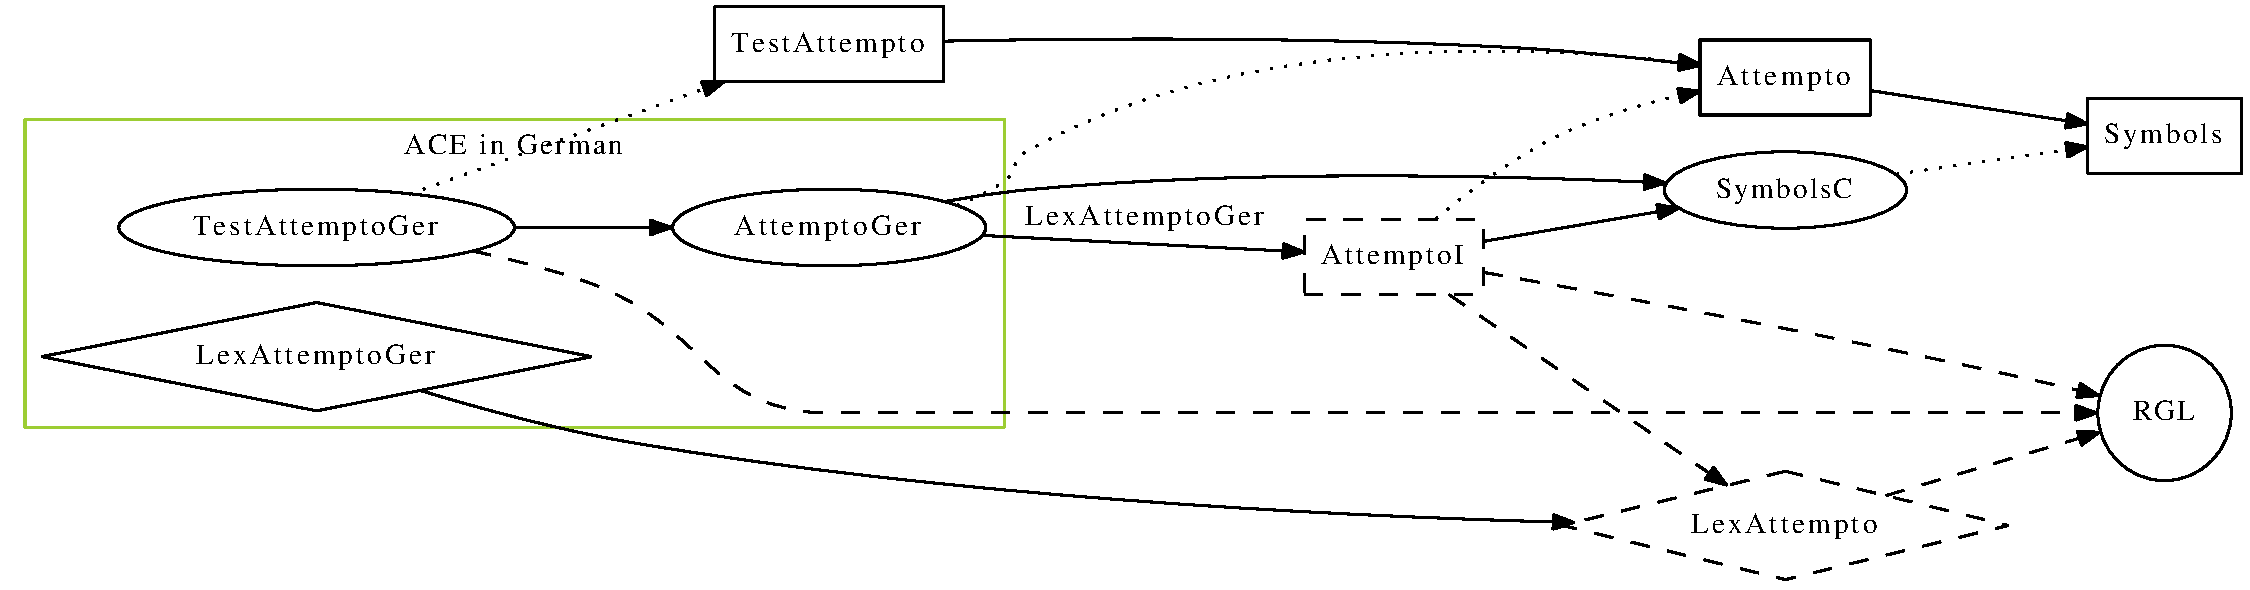
\includegraphics[width=0.99\textwidth]{modules}
\caption[Relations between the ACE grammar modules]
{Relations between the ACE grammar modules, using German (Ger) as an example
of one of the many concrete languages. To add support for a new language,
e.g. Dutch, one must implement three files:
\texttt{AttemptoDut}, which
instantiates the functor \texttt{AttemptoI} with Dutch-specific resources
from the RGL;
\texttt{TestAttemptoDut}, which contains the domain lexicon; and
\texttt{LexAttemptoDut}, which implements the Dutch-specific resources that
do not come from the RGL. The implementation of the lexicon can also
rely on the resources (Dutch morphological paradigms) implemented
in the RGL.}
\label{fig:modules}
\end{figure}

This architecture makes it easy to plug in support for new languages ---
one only needs to implement \texttt{Attempto\textit{Lan}} for the new language
\textit{Lan}. If the new language has RGL support and \texttt{AttemptoI}
already provides most of the implementation, then
the new module \texttt{Attempto\textit{Lan}} will be just a couple of lines
long.
(Note that the same idea is used in \cite{ranta:cnl2010_revised} to implement
a multilingual tourist phrasebook.)
This architecture makes it also easy to extend the grammar towards full ACE.
One needs to implement a set of new modules which import the existing modules
and add additional functions and their linearisations, and possibly
redefine existing functions if they implement restrictions that are not
present in full ACE.

The GF implementation follows the Codeco implementation, assigning a function
to each grammar rule unless it is too specific to ACE, in which case it
can be implemented as an ACE-only variant.
To correctly implement the ACE syntax, a new ACE-specific resource library
was created. For the most part it borrows all the operators from GF's English
resource library, but overrides certain constructions which in ACE have a
more specific form than in English, e.g. the ACE form for transitive
adjectives (`fond of') requires the preposition to be attached with
the hyphen (`fond-of'). The overall grammar thus treats ACE and English as
separate languages.

\subsection{Lexicon}

ACE makes a clear separation of lexicon and the rest of the syntax. The ACE
lexicon is a simple mapping of word forms to their corresponding lemmas, which
can be easily redefined by the users
\cite{ACE_6.6_Lexicon_Specification}. While the full ACE knows 27 types of
word forms (singular common noun, transitive verb, ...), the AceWiki subset
uses a smaller but also a slightly different set of lexical categories.

\begin{itemize}
\item proper name (with possible abbreviation and \emph{the}-prefix)
\item common noun (with singular and plural form)
\item noun in an \emph{of}-construct (e.g. `part', `child')
\item transitive verb (with 3rd singular, bare infinitive and past participle
forms)
\item transitive adjective (e.g. `fond-of')
\end{itemize}

GF does not make a clear separation between words and the rest of the grammar.
Furthermore, words can be described by complex structures holding information
about their gender, case, discontinuity, depending on the language. Most of
this necessary complexity is hidden by the RGL, which operates with common
lexical categories (e.g. \texttt{PN}, \texttt{V2}), and common and ``smart''
constructors (e.g. the simplest form of \texttt{mkN} takes one string as an
argument,
interprets this as the singular nominative form of the noun,
and guesses the remaining
unspecified information, e.g. the plural form and the gender).
Most of the ACE lexical categories are directly supported by the RGL and the
internal representations of words can be generated using RGL operators.
Table \ref{mapping_acewiki_to_gf} shows the mapping of AceWiki categories
to GF RGL English operators.

\begin{table}
\begin{center}
\begin{tabular}{ l l l }
\hline
AceWiki category & GF Cat & GF Eng oper \\
\hline
proper name & PN & \xp{mkPN john} \\
common noun & CN & \xp{mkCN (mkN sg pl)} \\
relational noun & CN & \xp{mkCN (mkN sg \_)} \\
transitive verb & V2 & \xp{mkV2 (mkV go goes \_ gone \_)} \\
transitive adjective & A2 & \xp{mkA2 (mkA fond) (mkPrep of)} \\
\hline
\end{tabular}
\end{center}
\caption{Mapping of AceWiki lexical categories
to GF RGL API categories and GF English
morphological paradigms. Underscore marks the omission of wordforms that
cannot occur in ACE but that are required by the GF RGL
operator. The AceWiki subset additionally
supports proper names which start with `the' (`the United Nations')
and abbreviated proper names (`the UN'),
the first feature can be handled by considering `the'
as a part of the proper name, the second can be implemented as a GF
variant.\protect\label{mapping_acewiki_to_gf}}
\end{table}

%Mapping the ACE lexical categories to GF RGL categories and morphological
%paradigms.
%[TODO: discuss variation]
%
%Table \ref{mapping_clex_to_gf} shows the mapping.
%
%\begin{table}
%\begin{center}
%\caption{Mapping of Clex to GF\protect\label{mapping_clex_to_gf}}
%\begin{tabular}{ r l l }
%\hline
%Clex & Cat & GF oper \\
%\hline
%\xp{noun\_mass} & MCN & \xp{mkCN (mkN ... (mkN ...))} \\
%\hline
%\end{tabular}
%\end{center}
%\end{table}


\section{Multilinguality}
\label{section:Multilinguality}

We included a number of different RGL-supported languages in the ACE-in-GF
implementation to discover the possible issues that a grammar engineer faces
when adding a new language. We also evaluated the resulting
translations for several of the included languages.
The currently included languages are
ACE,
Catalan,
Dutch,
English (almost identical to ACE),
Finnish,
French,
German,
Italian,
Spanish,
Swedish, and
Urdu.

The architecture described in section \ref{section:ACE_in_GF} not only
supports multilinguality but also makes implementing a new language in
the grammar relatively straight-forward provided that the language is
supported by the RGL. Adding a new language involves implementing all
the functions not present in \texttt{AttemptoI}, overriding the
\texttt{AttemptoI} implementation for functions which would otherwise
deliver a semantically or pragmatically wrong linearization,
implementing the few operators that are not provided by the RGL, and
providing the domain vocabulary for the application. Below are the
salient issues encountered during this process.

\paragraph{Non-universal constructs}
Some syntactic constructs described in the RGL are not present for all
languages, but provided as add-ons to the API via the \verb|Extra|
modules.  For our ACE implementation this is the case for VP
coordination, which does not exist in Urdu. This means that (ACE)
sentences which feature VP coordination could not be translated into
all the languages. An end-user application must therefore deal with
this issue, e.g. by asking the user to reformulate such sentences in a
way that preserves their meaning but uses a different syntactic
form. For example, VP coordination can be reformulated as relative
clause coordination --- ``John owns a car or owns a bike'' is in ACE
equivalent to ``John is somebody who owns a car or who owns a bike.''

\paragraph{Vocabulary}
The standard RGL lexicon of around 350 words could be used in certain
cases, but most of the time did not contain the words required for our
small application grammar. Some languages such as French and Swedish
do come with large dictionaries (in the order of tens of thousands of
words), however in general the work of porting the ACE grammar to new
languages requires the adding of at least some words. This is not
unusual when writing application grammars, however it must be noted
that writing such implementations requires knowledge of both the
language itself, and of how the smart paradigms provided for that
particular language work.

Most of the language implementations written for ACE were done so
\emph{without} the input of such language experts but merely on a
best-guess basis. For languages with which the developers are vaguely
familiar, the quality of the output produced is expected to be
fine, given that the correct GF smart paradigm is applied to the
correct wordform.
In the case of Urdu however, the unfamiliar script meant that adding words was
practically done blindly, so the quality of the translations from ACE to Urdu
is expected to be lower.

\paragraph{Low-level implementations}
One particular feature introduced in the ACE grammar is the use of a
pronoun as a noun phrase, which is used for handling ACE question sentences with
the \emph{wh}-word in the object position, e.g. ``Mary is a friend of who?''.
As no such coercion exists in the RGL, neither as
a straight function nor as a combination of multiple API constructors,
this conversion had to be implemented for each individual language.
In each case it required looking into the RGL source code for that language
to determine the linearisation types of each respective categories
and how one could be coerced into the other.
This work arguably oversteps the normal boundary within which application
grammarians are expected to work.

\paragraph{RGL inconsistencies}
Finally, the use of the RGL did uncover some inconsistencies between
language implementations. Specifically, the \verb|Numerals| module of
a number of languages in the RGL exposed many lexical categories which
they should not have, leading to conflicting category
inheritance. Furthermore, some languages were found to be incomplete,
in the sense that not all API functions were implemented. Such errors
in the RGL were patched accordingly so that work on the ACE
application grammar could continue.


\section{Evaluation}
\label{section:Evaluation}

In order to measure the quality of the grammar we can evaluate the following
properties.

\begin{description}
\item[Coverage]
i.e. how many syntactically correct ACE sentences does the grammar accept.
High coverage is required in applications which must translate a large variety
of ACE sentences. The goal is to have a 100\% coverage of the AceWiki subset.

\item[Precision]
i.e. how many syntactically incorrect ACE sentences does the grammar generate.
Over-generation is especially undesired in the context of look-ahead editing
\cite{schwitter:eamt-claw2003}, where users would be exposed to
forms which the actual language does not support.

\item[Ambiguity]
i.e. how many abstract trees are assigned on average to an accepted ACE
sentence. The goal is to parse each ACE sentence into to a single abstract
tree. However, some ambiguity can be tolerated if it is visible only internally,
and it does not result in multiple different translations.
That is if the ambiguity in one language is mapped to the same ambiguity in
another language.

\item[Multilingual correctness]
i.e. do the translations of an ACE sentence into other languages keep the
intended meaning of the original ACE sentence. Multilingual correctness allows
for knowledge engineering applications where users read and edit the underlying
knowledge base in multiple languages, understanding its content in the same
way regardless of the language.

\item[Performance]
i.e. how fast is the parser/lineariser. A minimal speed is required to embed
parsing and linearization into a user interface component, e.g. a look-ahead
editor.
\end{description}

In the following we mainly measure the grammar against the existing
Codeco grammar, and sometimes also against the full ACE Parsing Engine (APE).

\subsection{Syntactic coverage}

In order to test the syntactic coverage of the GF implementation of the
AceWiki subset we have used the AceWiki Codeco test set which
is an exhaustive set of sentences with length of up to 10
tokens \cite{kuhn2010doctoralthesis}. Each word
type is represented by a single word (e.g. `Mary' represents the proper name)
to make sure that all sentences are pairwise syntactically different, i.e.
do not differ only by choice of words.
The original test set contains 19718 sentences, but we removed sentences which
contain the `such that' construct which in ACE v6.6 is deprecated,
arriving at our test set of 19,422 sentences.
On the Codeco test set, our implementation successfully covers 100\% of the
sentences, however
a trade-off between syntactic coverage and ambiguity has been noted in the
grammar implementation. For more see section \ref{subsection:ambiguity}.

To measure the full ACE coverage, we used the $\sim$3000 sentences of the
APE regression test set. These are sentences and text
snippets that have been manually collected over several years. The sentences
can be of any length and use a large vocabulary, which we converted into
a GF grammar for the coverage test.
On the APE regression test set, our AceWiki-specific implementation covers
$\sim$50\% of full ACE.

\subsection{Syntactic precision}

To test the precision (i.e. possible over-generation) we have used the
random generation facility of the GF command line tool
(\verb!generate_random!). This allows us to randomly generate abstract
trees given the shape of the tree, its depth and its category. A
resulting tree can be then linearised as an ACE string which can be
parsed with a reference ACE parser.  This way of measuring precision
is somewhat unnatural as one cannot gradually go from shorter to
longer sentences --- at relatively low depths the sentences become
already so long and complex that checking them for the sources of
errors becomes cumbersome.

We measured the precision by randomly generating large numbers of
sentences at different tree depths and parsing them with both APE
and the Codeco parser. As a processing step after
generation but before parsing we rewrote the sentences to remove
illegal anaphoric references as these are not modelled in our grammar
as discussed in section \ref{subsection:Codeco}.  The precision values
obtained at various tree depths are shown in table
\ref{table:precision_scores}. It is clear from these results that the
precision of the grammar varies hugely according the depth of tree
used. Unfortunately we do not currently have any measure of how the grammar
precision degrades with sentence length.

In addition, the GF \verb!generate_random! function makes no
guarantees over the completeness of the generated trees'
coverage. Despite generating hundreds of trees in each test case, it
is very probable that some parts of the grammar are overused or
conversely untouched in the resulting test set.

\begin{table}
\begin{center}
\begin{tabular}{ c r r }
\hline
Depth & Avg. length & Precision (\%) \\
\hline
3 & 6 & 100.0 \\
4 & 11 & 98.0 \\
5 & 15 & 51.6 \\
6 & 23 & 40.8 \\
7 & 28 & 28.8 \\
\hline
\end{tabular}
\end{center}
\caption{Precision scores at various abstract syntax tree depths, as
  tested against the AceWiki subset reference parser. 500 sentences
  were generated and parsed in each case. The average sentence length
  in tokens is provided as an indication of
  sentence complexity.\protect\label{table:precision_scores}}
\end{table}

% "the precision was about 90\%" - not very clear since we are giving
% info about tree depth too
One should note that testing these generated sentences against full
ACE would hugely improve the precision measures, as the AceWiki subset
sets several restrictions on the sentence patterns that it supports,
e.g. a negated NP is not allowed in existential sentences (`there is
nobody'), an NP with a generalised quantifier cannot take a relative
clause (`less than 3 men that own a car`). The AceWiki subset also
does not support some variants (e.g. the contracted forms such as
`isn't' and `doesn't').  We decided not to restrict our grammar in a
similar fashion as this would have caused a blowup of grammar
rules. This relaxing of restrictions and introduction of syntactic
sugar makes our implementation deviate somewhat from the AceWiki subset
and move it closer towards full ACE.
These deviations are often actually still compatible with the
subset of ACE that can be mapped to OWL, which is the main motivation
of the AceWiki subset as well. In other words, the case could be
made for actually including these constructs to the AceWiki subset, rather
than restricting the GF implementation.

%There are also
%places where the AceWiki subset could be extended (rather that its GF
%implementation restricted), e.g. AceWiki currently rejects ``every man
%likes less than 3 men that own a cat.'' because an NP with a
%generalized quantifier (less than 3) cannot be followed by a relative
%clause. But this sentence is supported by the ACE-OWL translator
%so there is no real reason why it should not be allowed in the
%AceWiki subset.

% AceWiki does support: ``... that Mary likes``
%Also, support for object relative clauses (``.. that Mary is mad-about'')
%is desirable (even though AceWiki does not completely support it).

% AceWiki does not support: who does Mary (not) like?
% (only: Mary likes (does not like) who?)

\subsection{Ambiguity}
\label{subsection:ambiguity}

We measured the occurrence of ambiguous parses also on the Codeco test set,
and were able to achieve an ambiguity level as low as 3.3\%.
In these relatively rare cases, the grammar assigns two abstract trees
to an input ACE sentence. This is always semantically harmless ambiguity
(i.e. it would not manifest itself in translations) resulting from the rules
for common nouns and noun phrases which accept similar input structures.

However a distinct trade-off between syntactic coverage and ambiguity
has been noted in our implementation.  Specifically, the single rule
covering the `there is' construct, for example ``there is somebody
who is a woman'' covers 159 sentences from the test set (0.8\%), but
also pushes the ambiguity down by over 10\%. In other words, we are
able to achieve 99.2\% coverage with 3.3\% ambiguity, or 100\%
coverage but with 13.6\% ambiguity, but retaining full coverage while
bringing the ambiguity down proved to be problematic.

%% [TODO: analyse better the reasons for ambiguity,
%% most of it seems to be spurious ambiguity,
%% but there are also cases like
%% ``for every  woman  there is  somebody  and  there is  somebody  .'',
%% .]

Having some numeric indication of ambiguity is one thing, however
properly understanding the source of such ambiguities is a less
obvious task. Ambiguities occur in grammars when separate rules or
chains of rules have the same effective type signature. For example,
attempting to parse the sentence fragment ``a woman who asks Mary''
returns two viable GF parse trees:

{\footnotesize
\begin{verbatim}
aNP (relCN (cn_as_VarCN woman_CN) (predRS which_RP (v2VP ask_V2 (pnNP mary_PN))))
relThereNP (aNP (cn_as_VarCN woman_CN)) (predRS which_RP (v2VP ask_V2 (pnNP mary_PN)))
\end{verbatim}
}

As in the ACE parser itself, such a fragment should only have a single
parse tree, which corresponds to the former tree given above. This
indicates some undesired generality in the \verb|relThereNP| function,
which should clearly be factored out of the grammar. However the task
of removing ambiguity while preserving coverage is non-trivial,
requires a close analysis of the problem cases and an understanding of
the grammar as a whole.
It should also be noted that the Codeco test set used might be
too small to reveal certain kinds of ambiguities; the measure of precision we
have is only as good as our test set, which was not specifically designed for
testing such grammar attributes.

\subsection{Multilinguality}

To test the correctness of the multilingual translations we have used
the ACE sentences from the
Ontograph
Framework\footnote{\url{http://attempto.ifi.uzh.ch/site/docs/ontograph/}}
\cite{kuhn2009cnlmain}. The selected 40 sentences cover all main sentence
patterns of the AceWiki subset and have been used before in user
evaluations of how well the users understand the precise formal meaning of ACE.
The sentences have a very clear set-theoretic meaning, e.g.
``Everything that is a traveler or that is an officer sees
at most 1 aquarium.'' means that the union of the sets \emph{traveler} and
\emph{officer} is a subset of the set of all instances that participate in
the 1st argument position in at most one \emph{sees}-relation with an
instance from the set \emph{aquarium}.
The hypothesis to be confirmed is whether this meaning is understood in
the same way via all the languages.

While the tests of coverage and precision can be automated, the test
of multilingual correctness requires that (native) speakers of the
evaluated languages manually check the translations. We set up a
Google Docs form that presents the list of 40 sentences each
translated into 9 languages (Catalan, Dutch, Finnish, French, German,
Italian, Spanish, Swedish and Urdu), and asked native speakers of
these languages to check the list and report the syntactic, semantic
and pragmatic (naturalness) errors in the sentences.  In order to
judge the semantic correctness of the translations, the evaluator must
also consider the original ACE sentence. The evaluation form therefore
comes with a short description of ACE and its interpretation rules
that are relevant for the presented sentences.

The evaluation provided valuable native speaker feedback that will
allow us to correct various morphological and syntactic errors. It
also pointed out some semantic issues, which can be mostly fixed by
making language-specific customisation to the grammar. In the worst
case, if an ACE construct cannot be made available in a language, then
it would generate a zero-linearization which would inform the grammar
user that this construct is not available in all the languages and
therefore should not be used. ACE offers some amount of syntactic
sugar, so sentences can usually be reformulated. This was the case for
VP-coordination in Urdu, where the evaluators were asked to ignore the
lack of translations caused by the missing support for the construct.
The issues arising from this preliminary evaluation step are described
below.

\paragraph{RGL Errors}
A few errors in the test linearisations were traced to errors in the
Resource Grammar Library, and not in the Attempto grammar itself.
These included indefinite article and other missing articles in Urdu,
and the plural indefinite accusative case in Finnish.


\paragraph{Incorrect use of smart paradigms}
Other mistakes in the test sentences were caused by using the RGL's
smart paradigms with incorrect input forms. For example
\verb|mkN "matkustajan"| (genitive) instead of the correct form
\verb|mkN "matkustaja"| (nominative) in Finnish. Such errors are easy to fix,
however they underscore the need for language experts who are familiar
with the smart paradigms in the RGL, even when implementing minor
vocabularies such as in our case. This problem was even more
pronounced in the case of Urdu, where the grammar developers did not
have any knowledge of the language's script, let alone its vocabulary.

% Word order problems in Urdu when combining Roman/Persian scripts

\paragraph{Stylistic issues}
In Finnish for example, for human nouns like ``mies'' (man), it is
preferable to use the pronoun ``kukaan'' instead of ``mikään''. This
could be solved by a feature saying if a noun is (semantically)
human. Moreover, this is not true in all positions: ``John is no
golfer'' should be ``John ei ole mikään golfaaja'', so getting this
correct would require significantly more work and language-expert
input than initially used.  However it should be noted that this lack
of distinction is actually a limitation in the AceWiki subset itself.

Negation in German also raised some issues amongst the evaluators.  An
initial bug in the grammar produced the sentence ``Bill ist ein Golfer
nicht'', which is grammatically wrong.  Fixing this gave the new
sentence ``Bill ist nicht ein Golfer'', which is grammatically
acceptable, but pragmatically questionable.  The only truly correct
translation into German is ``Bill ist kein Golfer'', however this
would then create an ambiguity between ``Bill isn't a golfer'' and
``Bill is no golfer'',
which are distinct ACE sentences having distinct DRSs,
though these are interpreted as semantically equivalent.


\paragraph{Negative determiners}

Perhaps the biggest issue brought up through this evaluation was the
use of negative determiners, e.g. ``no man''.  Translating such
determiners on a syntactic level can easily result in meaning shifts
between languages, if the grammar author is not careful. The problem
is that the translations do not always preserve the meaning of
sentences like:
\begin{itemize*}
  \item every man loves a woman .
%  \item every man loves no woman .
%  \item every man does not love a woman .
  \item every man does not love no woman .
%  \item no man loves a woman .
  \item no man loves no woman .
  \item no man does not love a woman .
%  \item no man does not love no woman .
\end{itemize*}
Some of which in ACE are semantically equivalent either because they
have the exact same (i.e. lexically identical) DRS, or because they
have DRSs which are interpreted as equivalent in first order logic.

% ACE sentences with double negation for instance ``no man loves no
% woman'' have different meanings in different languages, and also
% their syntax can be rather special.

Finnish for example has no equivalent of the \emph{no} determiner, but
has to express it with \emph{any} and \emph{not}.  Thus ``no
man is a golfer'' must be paraphrased as ``any man is not a golfer''
(``mikään mies ei ole golfaaja''), and ``John knows no golfer'' must
become ``John doesn't know any golfer'' (``John ei tunne mitään
golfaajaa'').  If you apply this to a sentence with two such
determiners, you end up converting ``no man knows no woman'' into
``any man doesn't know any woman'' (``mikään mies ei tunne mitään
naista''), which means that no double negation is created.
The situation is similar in the Romance languages,
% no man is a golfer -> aucun homme n'est un golfeur
% no man loves a woman -> aucun homme n'aime aucune femme
confirming that negative determiners are a problem in a multilingual
setting, if compositional semantics is desired.

This was eventually handled by extending the RGL to include noun
phrase polarity.  The idea is that NP's have a boolean feature
\verb|isNeg|, which tells if the element is negative (e.g. `nobody', `no
man'). If any NP in a clause is negative, the \textbf{positive} form of
the clause gets a negation. Thus in Italian ``nobody sleeps'' becomes
``nessuno non dorme'', whereas ``no man sees nothing'' is translated
to ``nessun uomo non vede niente''.  In French, the negation without
\emph{pas} is used, i.e. becoming ``personne ne dort'' and ``aucun
homme ne voit rien'' respectively.
%% Notice that if there are two negative elements, the natural interpretation
%% changes. As a variant of this principle, if the English sentence has a
%% negation, it has no effect on the Italian sentence:
%%   nobody doesn't sleep -> nessuno non dorme
%% In French, nowever, the "stronger" ("ordinary") negation is then used:
%%   personne ne dort pas
%% which can be interpreted as a double negation.
However although this creates grammatical translations in all cases,
in sentences which contain more than one negative element, the
semantic meaning changes.

In the case of German, this can be achieved either through sentence
negation or noun phrase negation as above.
% - sentence negation: ich habe einen Menschen gesehen ->
%   ich habe nicht einen Menschen gesehen, \verb|mkS negativePol (...a_Det...)|
% - noun phrase negation: ich habe keinen Menschen gesehen,
%   \verb|mkS positivePol (...no_Det...)|
This is up to the application grammarian to select the type of
negation desired, which of course requires a good intuition on German.
Dutch has similar problems with \emph{geen} and \emph{niet}, and
moreover the placing of \emph{niet} is sometimes different from
German.

\paragraph{Suitability of test set}

The Ontograph test set was originally not developed to evaluate multilingual
correctness. Therefore, a future evaluation should use a more customized
set of sentences, e.g. which takes the distinctive features of each language
into account.
Also the current set of 40 sentences did not contain some important ACE
constructs, e.g. questions and sentence negation.

%[TODO: this was covered to some extent by the Help-sheet that accompanied
% the evaluation]
%does not cover some core ACE equivalences,
%e.g. \emph{if-then} equals \emph{every}, double negation equals no negation.
%How are these equivalences preserved under the direct syntax-based
%translation?

\paragraph{Evaluation format}
Using a spreadsheet to tabulate the linearised sentences along with
the evaluator's feedback was quick and easy to do, but some
dissatisfaction was expressed over the inconvenience with the
layout. Even with this relatively small test set, it was clear that
more effort must be put into evaluation interfaces in order to make
the most out of human evaluators.

\subsection{Performance}

We measured the performance of the grammar implementation on an i3 laptop
with 4GB of RAM.
The implementation is relatively fast, being capable of parsing
all 19,422 Codeco test sentences in 55 seconds
(i.e. 353 sentences/sec). In comparison, the Codeco parser (transformed into
Definite Clause Grammar and executed by SWI-Prolog) parses
the same set in 25 seconds.
(Note that we did not measure the performance of parsing languages other than
ACE.)
In order to linearize the
resulting parse trees into 11 languages an additional 30 seconds is needed.
The linearization speed does not depend on the target language.

In general,
the measured performance enables applications where a relatively large ACE
knowledge base is stored as a set of GF abstract trees and linearised into a
multilingual presentation on demand in a few minutes. It also supports
interactive applications that include look-ahead editing.

\section{Conclusions and future work}
\label{section:Conclusions}

We have presented a set of GF grammar modules that implement the AceWiki
subset of ACE and make it available in multiple natural languages. The design
of the grammar makes it easily extendable to more languages and to a larger
coverage of ACE.
We have also described the main differences between the grammar formalisms
of Codeco (in which the AceWiki subset is originally defined) and GF. Directly
translating the Codeco grammar to GF proved to be impossible which made the
engineering of the AceWiki subset in GF non-trivial and a fully
precise grammar could not be obtained.
We have also described a testing and evaluation framework that can be used
during and after the development.

Future work includes plugging in new languages as support for them becomes
available in the RGL as well as adding more ACE constructs. We also plan
to use the developed grammar as a module in the AceWiki semantic wiki system
to power the look-ahead editor and offer multilingual viewing and editing
of the wiki content. Using the grammar in an actual application also offers
new ways to evaluate the notion of multilingual controlled natural language.

\section*{Acknowledgement}

We would like to thank
Olga Caprotti,
Tobias Kuhn,
K.V.S. Prasad,
Aarne Ranta,
Jordi Saludes,
and
Shafqat Virk
for their time in completing our
evaluation and the valuable contributions they provided.

\bibliography{bib}
\bibliographystyle{alpha}
%\bibliographystyle{plain}

\end{document}

% Recycle Bin follows
\begin{itemize}
\item ACE is written in the unification style vs. GF grammar is written
by separating the abstract syntax from the concrete
\item ACE offers support for anaphoric references (a feature present in most
logical rule and ontology languages) vs. GF does not provide similar support
\end{itemize}
